% Choose one to switch between slides and handout
%\documentclass[]{beamer}
\documentclass[handout]{beamer}

% Video Meta Data
\title{Bitcoin, Blockchain and Cryptoassets}
\subtitle{The Bitcoin Network}
\author{Prof. Dr. Fabian Schär}
\institute{University of Basel}

% Config File
% Packages
\usepackage[utf8]{inputenc}
\usepackage{hyperref}
\usepackage{gitinfo2}
\usepackage{tikz}
\usepackage{amsmath}
\usepackage{mathtools}
\usepackage{bibentry}
\usepackage{xcolor}
\usepackage{colortbl} % Add colour to LaTeX tables
\usepackage{caption}
\usepackage[export]{adjustbox}
\usepackage{pgfplots} \pgfplotsset{compat = 1.17}
\usepackage{makecell}
\usepackage{fancybox}
\usepackage{ragged2e}
\usepackage{fontawesome}
\usepackage{seqsplit}
\usepackage{tabularx}

% Color Options
\definecolor{highlight}{rgb}{0.65,0.84,0.82}
\definecolor{focus}{rgb}{0.72, 0, 0}
\definecolor{lightred}{rgb}{0.8,0.5,0.5}
\definecolor{midgray}{RGB}{190,195,200}

% Beamer Template Options
\beamertemplatenavigationsymbolsempty
\setbeamertemplate{footline}[frame number]
\setbeamercolor{structure}{fg=black}
\setbeamercolor{footline}{fg=black}
\setbeamercolor{title}{fg=black}
\setbeamercolor{frametitle}{fg=black}
\setbeamercolor{item}{fg=black}
\setbeamercolor{}{fg=black}
\setbeamercolor{bibliography item}{fg=black}
\setbeamercolor*{bibliography entry title}{fg=black}
\setbeamercolor{alerted text}{fg=focus}
\setbeamertemplate{items}[square]
\setbeamertemplate{enumerate items}[default]
\captionsetup[figure]{labelfont={color=black},font={color=black}}
\captionsetup[table]{labelfont={color=black},font={color=black}}

\setbeamertemplate{bibliography item}{\insertbiblabel}

% Link Icon Command
\newcommand{\link}{%
    \tikz[x=1.2ex, y=1.2ex, baseline=-0.05ex]{%
        \begin{scope}[x=1ex, y=1ex]
            \clip (-0.1,-0.1)
                --++ (-0, 1.2)
                --++ (0.6, 0)
                --++ (0, -0.6)
                --++ (0.6, 0)
                --++ (0, -1);
            \path[draw,
                line width = 0.5,
                rounded corners=0.5]
                (0,0) rectangle (1,1);
        \end{scope}
        \path[draw, line width = 0.5] (0.5, 0.5)
            -- (1, 1);
        \path[draw, line width = 0.5] (0.6, 1)
            -- (1, 1) -- (1, 0.6);
        }
    }

% Read Git Data from Github Actions Workflow
% Defaults to gitinfo2 for local builds
\IfFileExists{gitInfo.txt}
	{\input{gitInfo.txt}}
	{
		\newcommand{\gitRelease}{(Local Release)}
		\newcommand{\gitSHA}{\gitHash}
		\newcommand{\gitDate}{\gitAuthorIsoDate}
	}

% Custom Titlepage
\defbeamertemplate*{title page}{customized}[1][]
{
  \vspace{-0cm}\hfill\includegraphics[width=2.5cm]{../config/logo_cif}
  \includegraphics[width=1.9cm]{../config/seal_wwz}
  \\ \vspace{2em}
  \usebeamerfont{title}\textbf{\inserttitle}\par
  \usebeamerfont{title}\usebeamercolor[fg]{title}\insertsubtitle\par  \vspace{1.5em}
  \small\usebeamerfont{author}\insertauthor\par
  \usebeamerfont{author}\insertinstitute\par \vspace{2em}
  \usebeamercolor[fg]{titlegraphic}\inserttitlegraphic
    \tiny \noindent \texttt{Release Ver.: \gitRelease}\\ 
    \texttt{Version Hash: \gitSHA}\\
    \texttt{Version Date: \gitDate}\\ \vspace{1em}
    
    
    \iffalse
  \link \href{https://github.com/cifunibas/Bitcoin-Blockchain-Cryptoassets/blob/main/slides/intro.pdf}
  {Get most recent version}\\
  \link \href{https://github.com/cifunibas/Bitcoin-Blockchain-Cryptoassets/blob/main/slides/intro.pdf}
  {Watch video lecture}\\ 
  
  \fi
  
  \vspace{1em}
  License: \texttt{Creative Commons Attribution-NonCommercial-ShareAlike 4.0 International}\\\vspace{2em}
  \includegraphics[width = 1.2cm]{../config/license}
}


% tikzlibraries
\usetikzlibrary{decorations.pathreplacing}
\usetikzlibrary{decorations.markings}
\usetikzlibrary{positioning}
\usetikzlibrary{calc}
\captionsetup{font=footnotesize}


%%%%%%%%%%%%%%%%%%%%%%%%%%%%%%%%%%%%%%%%%%%%%%
%%%%%%%%%%%%%%%%%%%%%%%%%%%%%%%%%%%%%%%%%%%%%%

\begin{document}

\thispagestyle{empty}
\begin{frame}[noframenumbering]
	\titlepage
\end{frame}

%%%
\begin{frame}{Bitcoin is a Peer-to-Peer Network}
	\centering
	\begin{tikzpicture}[scale=1, every node/.style={scale=1}]
		
% Title
%\node[above] at (2,4.3) {Peer-to-Peer};


% Network
\node (agenta) at (1,2.8) {\includegraphics[width = 0.6 cm]{../assets/images/agents/avatar_rand3.png}};
\node (agentb) at (0.5,1) {\includegraphics[width = 0.6 cm]{../assets/images/agents/avatar_rand4.png}};
\node (agentc) at (3,2.1) {\includegraphics[width = 0.6 cm]{../assets/images/agents/avatar_rand5.png}};
\node (agentd) at (2.8,0) {\includegraphics[width = 0.6 cm]{../assets/images/agents/avatar_rand1.png}};
\node (agente) at (5,4.3) {\includegraphics[width = 0.6 cm]{../assets/images/agents/avatar_rand2.png}};	
\node (agentf) at (5.1,1.1) {\includegraphics[width = 0.6 cm]{../assets/images/agents/avatar_rand3.png}};
\node (agentg) at (7.5,3.8) {\includegraphics[width = 0.6 cm]{../assets/images/agents/avatar_rand4.png}};
\node (agenth) at (6.7,0.4) {\includegraphics[width = 0.6 cm]{../assets/images/agents/avatar_rand5.png}};

% Network flow
\draw[<->, thick, dashed]	(agenta.south) -- (agentb.north);
\draw[<->, thick, dashed] 	(agenta.east) -- (agente.west);
\draw[<->, thick, dashed]	(agenta.south east) -- (agentc.west);
\draw[<->, thick, dashed]	(agente.south west) -- (agentc.north east);
\draw[<->, thick, dashed]	(agente.south) -- (agentf.north);
\draw[<->, thick, dashed]	(agente.east) -- (agentg.west);
\draw[<->, thick, dashed]	(agentc.south west) -- (agentb.east);
\draw[<->, thick, dashed]	(agentc.south) -- (agentd.north);
\draw[<->, thick, dashed]	(agentc.south east) --  (agentf.west);
\draw[<->, thick, dashed]	(agentg.south west) -- (agentf.north east);
\draw[<->, thick, dashed]	(agentg.south) -- (agenth.north);
\draw[<->, thick, dashed]	(agentb.south east) -- (agentd.west);
\draw[<->, thick, dashed]	(agentf.south west) -- (agentd.east);
\draw[<->, thick, dashed]	(agentf.south east) -- (agenth.west);
\draw[<->, thick, dashed]	(agenth.south west) -- (agentd.east);

	\end{tikzpicture}
	
	\vspace{0.5cm}
	
	In the Bitcoin network, participants are called \color{focus}nodes\color{black}.
\end{frame}
%%%

%%%
\begin{frame}{Joining the Network}
	\begin{center}
		\begin{tikzpicture}[scale=1, every node/.style={scale=1}]
			\begin{footnotesize}

	\node (install) at (0, 0) {
\includegraphics[height = 0.15\textheight]{../assets/images/server}};
	\node[below = 2pt] at (install.south) {Install Client};
	
	\node (peer) at (8, 0) {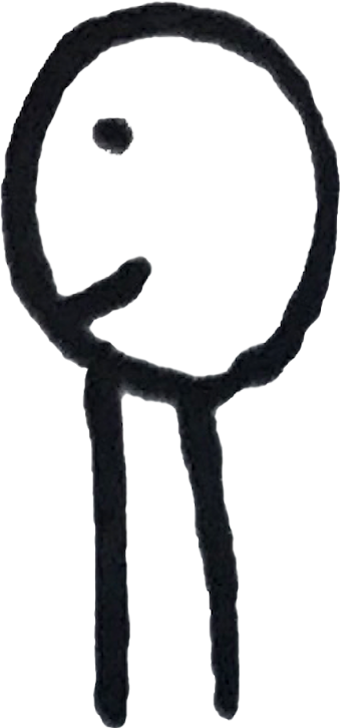
\includegraphics[height = 0.15\textheight]{../assets/images/agents/agent_left}};
	
	\draw[->, thick] ([yshift=5pt]install.east) -- node[midway, above = 3pt] {version} ([yshift=5pt]peer.west);
	\draw[<-, thick] ([yshift=-5pt]install.east) -- node[midway, below = 3pt] {verack} ([yshift=-5pt]peer.west);
	
\end{footnotesize}
		\end{tikzpicture}
	\end{center}

	\vspace{1cm}
	
	After the initial handshake, we request a list of IP addresses and connect to additional peers.
\end{frame}
%%%

%%%
\begin{frame}{Functionality of a Full Node}
	\centering
	\begin{tikzpicture}[scale=1, every node/.style={scale=1}]
		\begin{footnotesize}
	\coordinate (1) at (-4, 3);
	\coordinate (2) at (0, 3);
	\coordinate (3) at (4, 3);
	\coordinate (4) at (-2, 0);
	\coordinate (5) at (2, 0);
	
	\coordinate (a) at (-5.3, 4);
	\coordinate (b) at (5.3, 2);
	\filldraw[fill=highlight] (a) rectangle (b);
	\node at (0, 4.2) {Core Functionality};
	
	\coordinate (c) at (-5.3, 1);
	\coordinate (d) at (5.3, -1);
	\filldraw[fill=highlight!30!white, dotted] (c) rectangle (d);
	\node at (0, 1.2) {Optional Functionality};
	
	\node at (1) {
\includegraphics[height = 0.1\textheight]{../assets/images/copy}};
	\node[below = 14pt] at (1) {Copy of Ledger};
	
	\node at (2) {
\includegraphics[height = 0.1\textheight]{../assets/images/verify}};
	\node[below = 14pt] at (2) {Verify};
	
	\node at (3) {
\includegraphics[height = 0.1\textheight]{../assets/images/forward}};
	\node[below = 14pt] at (3) {Distribute};
	
	\node at (4) {
\includegraphics[height = 0.1\textheight]{../assets/images/wallet}};
	\node[below = 14pt] at (4) {Wallet};
	
	\node at (5) {
\includegraphics[height = 0.1\textheight]{../assets/images/pickaxe}};
	\node[below = 14pt] at (5) {Mining};
	
	
\end{footnotesize}
	\end{tikzpicture}
\end{frame}
%%%


%%%
\begin{frame}{Verify New Blocks}
	
	\begin{tikzpicture}[scale=1, every node/.style={scale=1}]
		\begin{footnotesize}
	
	\node (ledger) at (0, 3) {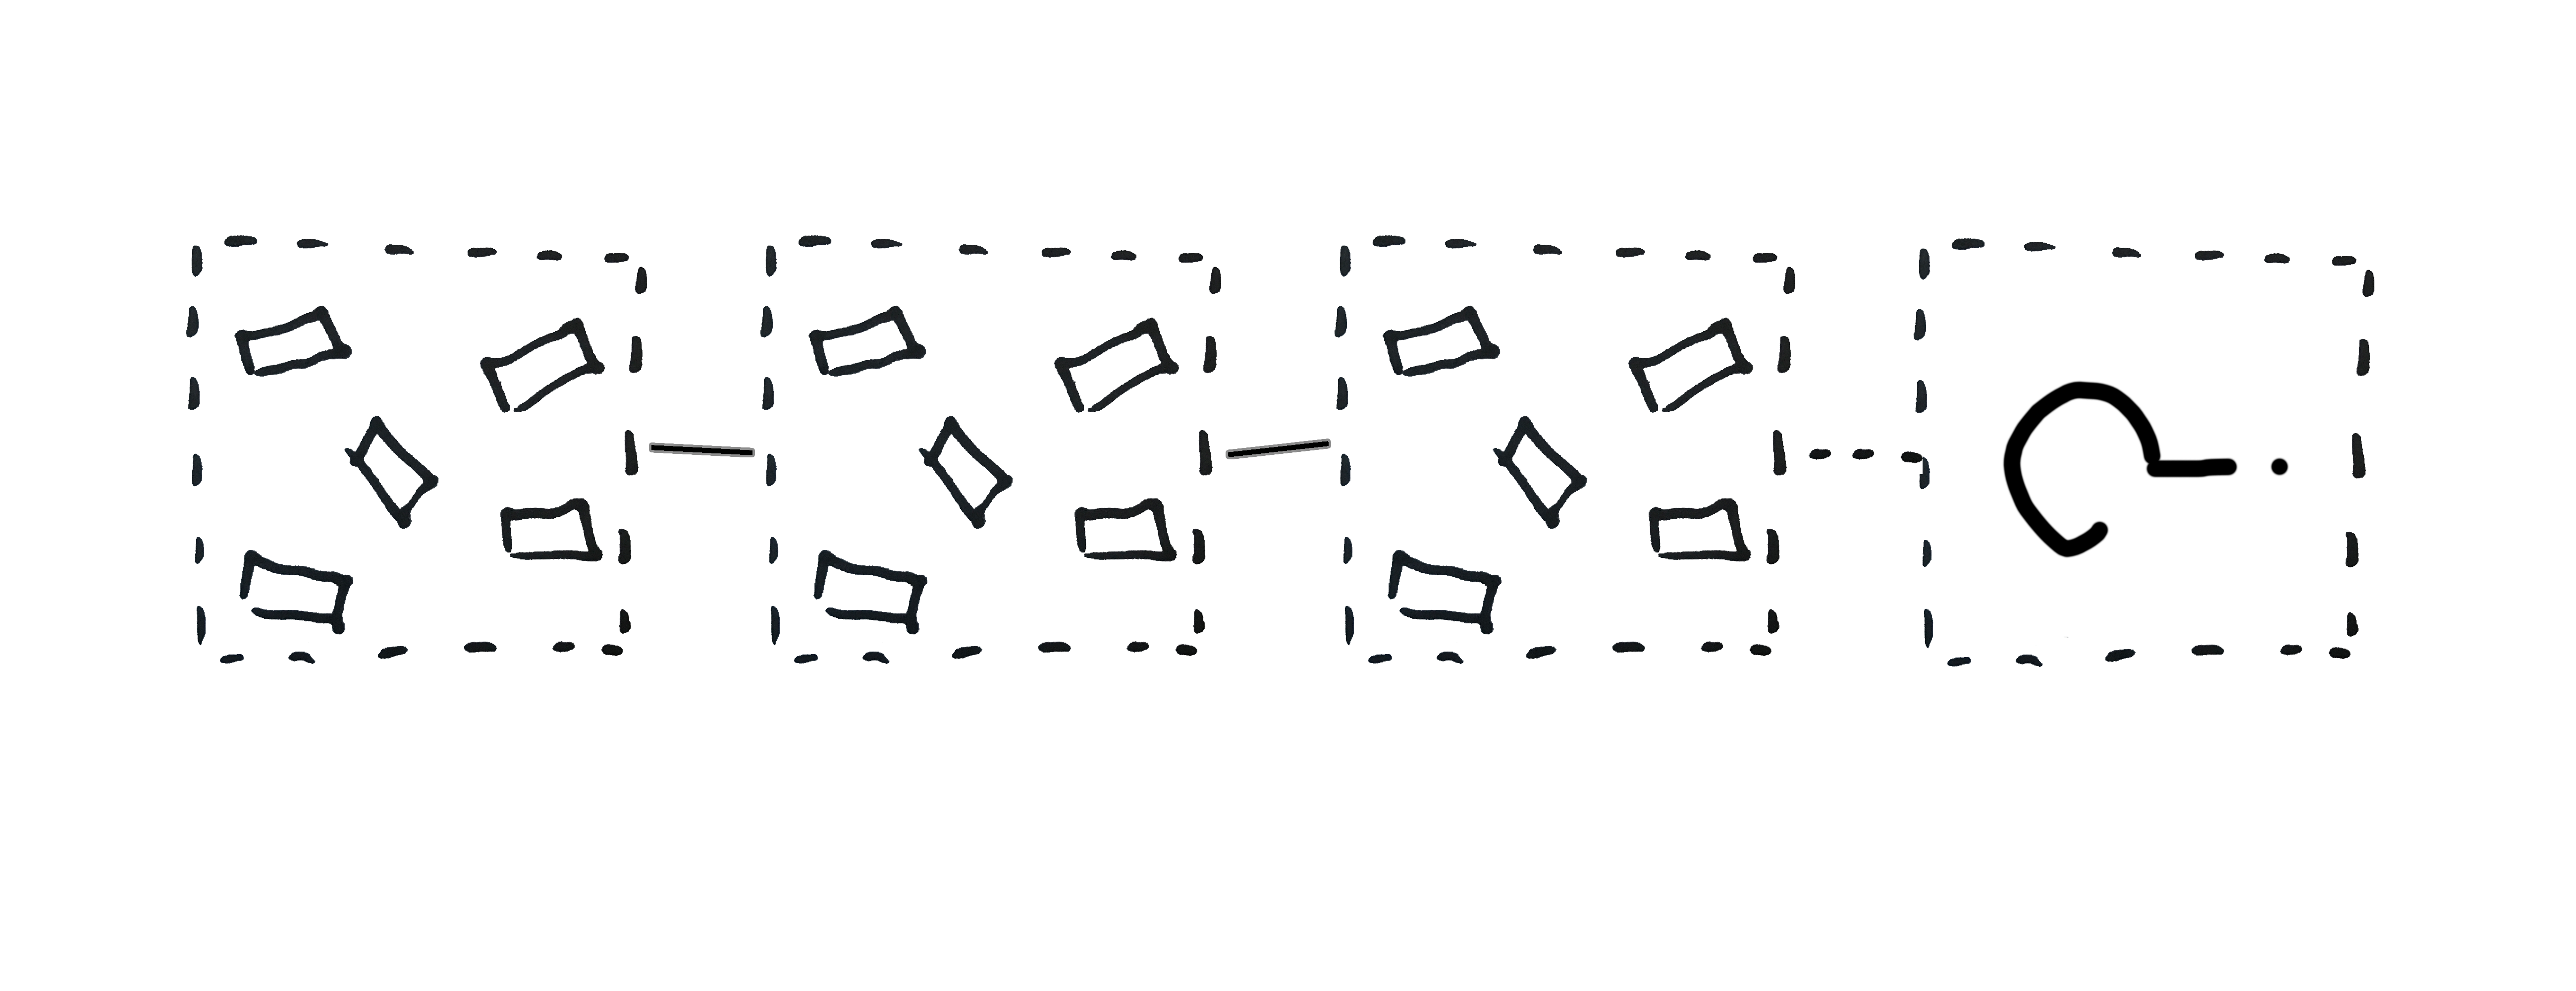
\includegraphics[height = 0.3\textheight, rotate = -90]{../assets/images/blocks_4}};
	\node (client) at (2, 3) {
\includegraphics[height = 0.2\textheight]{../assets/images/agents/agent_right}};
	\node (agent1) at (6, 5) {
\includegraphics[height = 0.2\textheight]{../assets/images/agents/handing_left}};
	\node (block1) at (agent1) {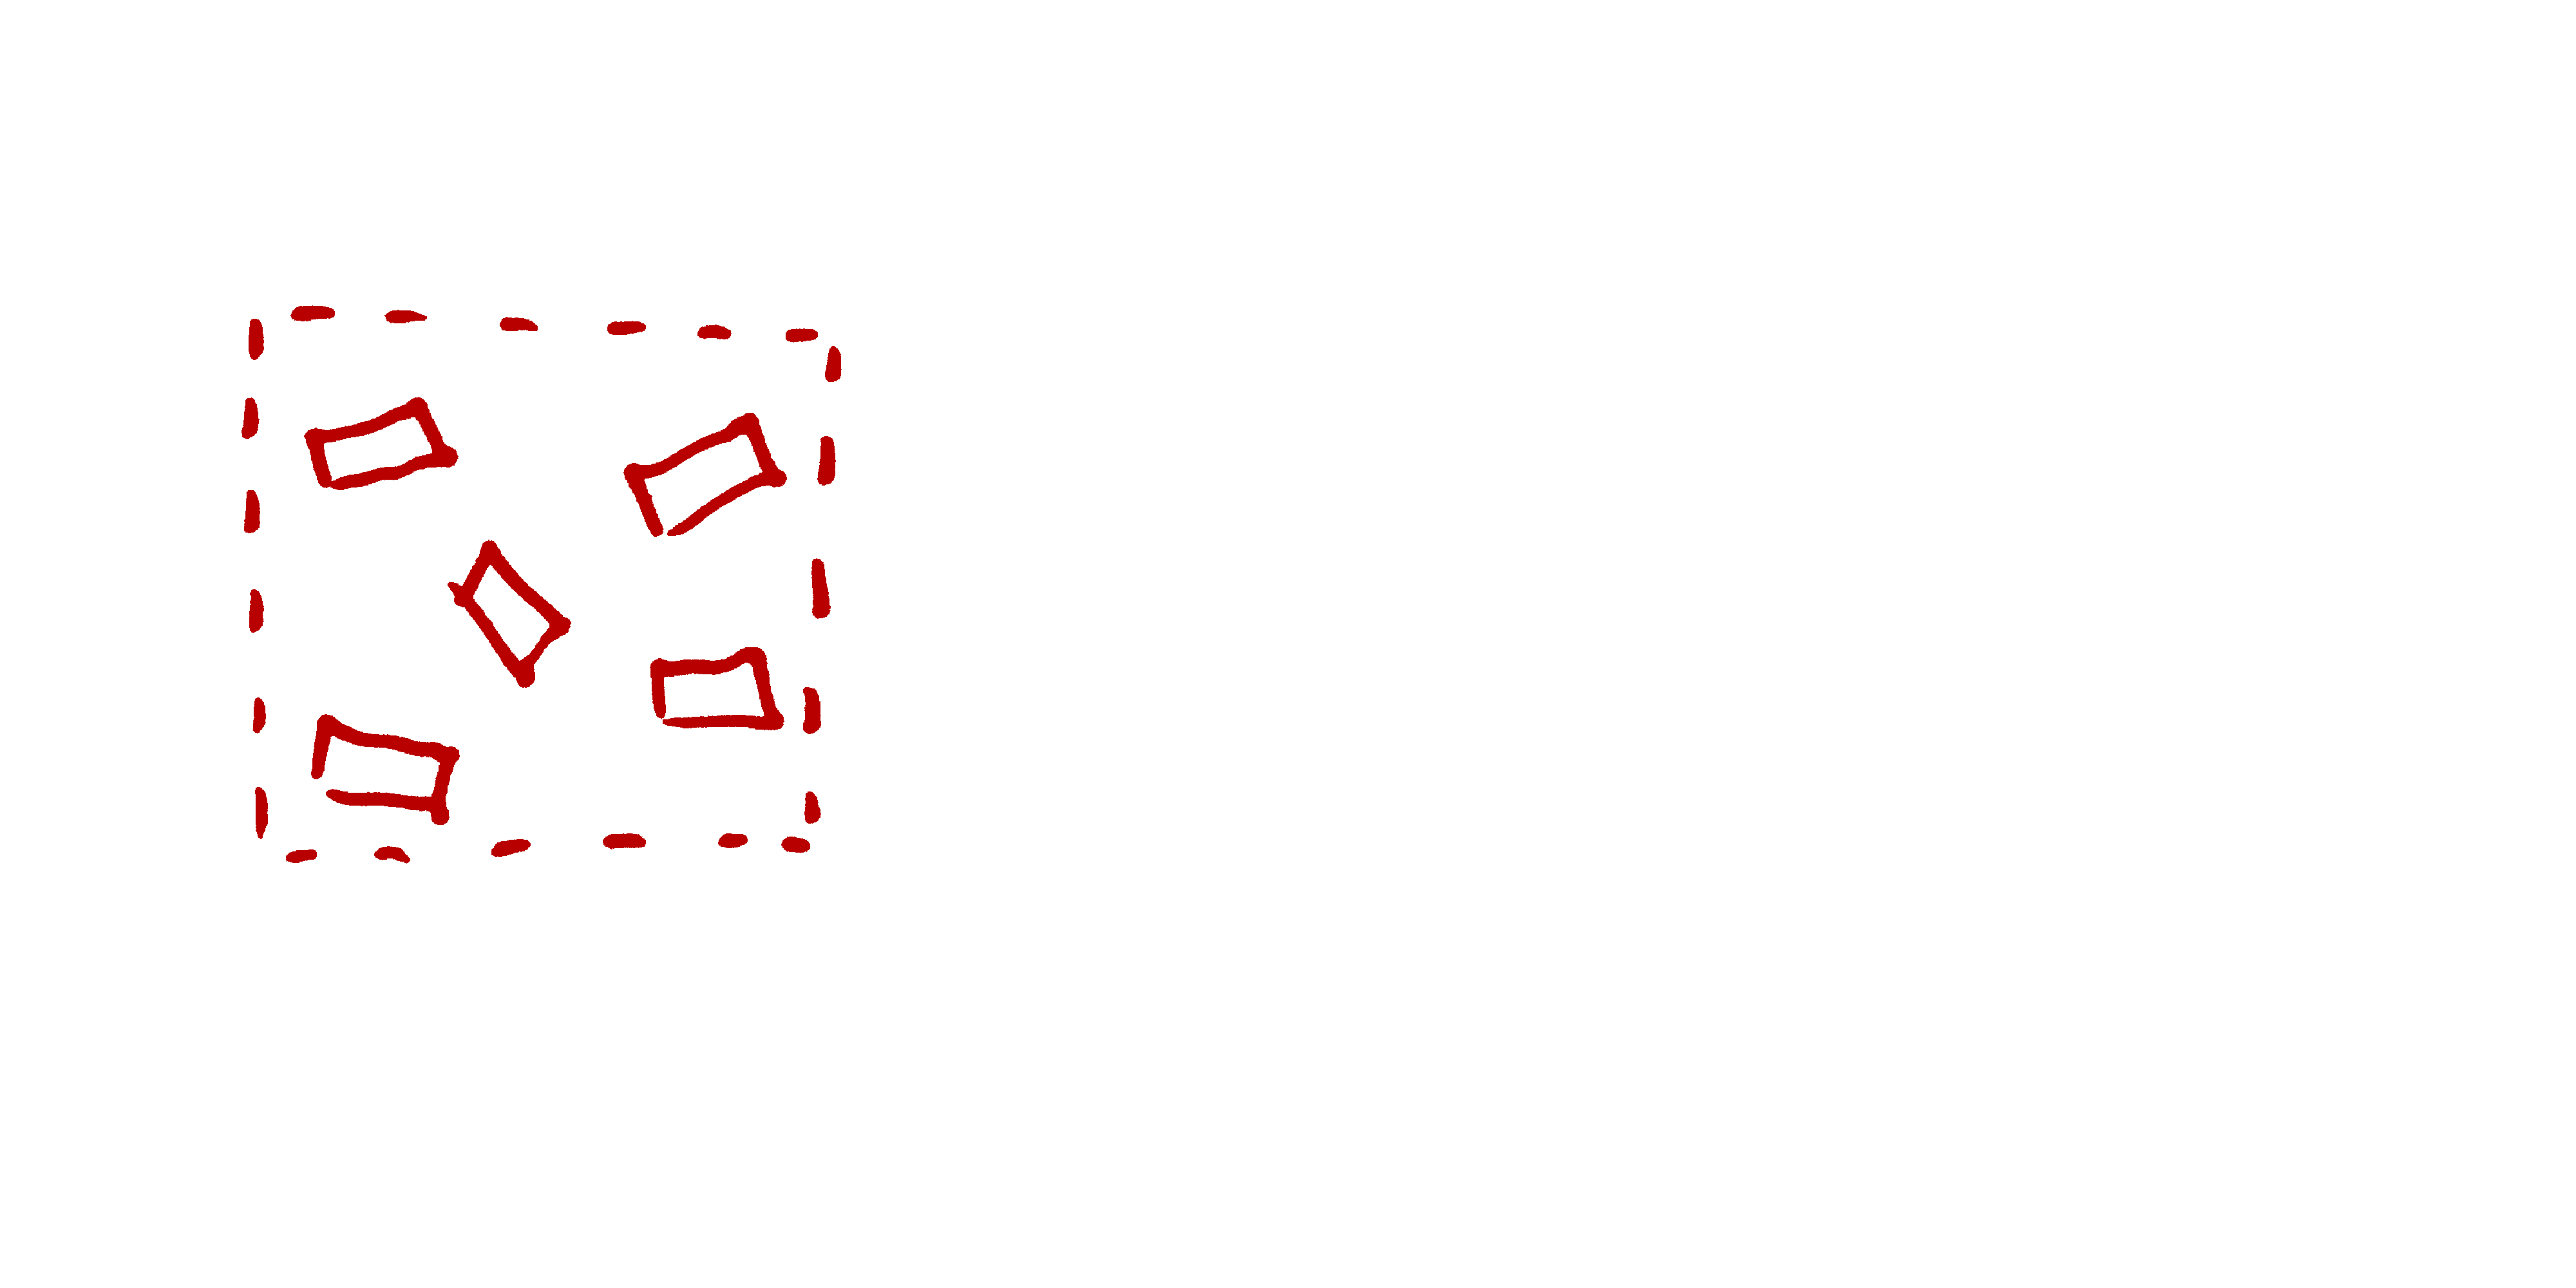
\includegraphics[height = 0.3\textheight]{../assets/images/block_1_red}};
	\node (agent2) at (6, 1) {
\includegraphics[height = 0.2\textheight]{../assets/images/agents/handing_left}};
	\node (block2) at (agent2) {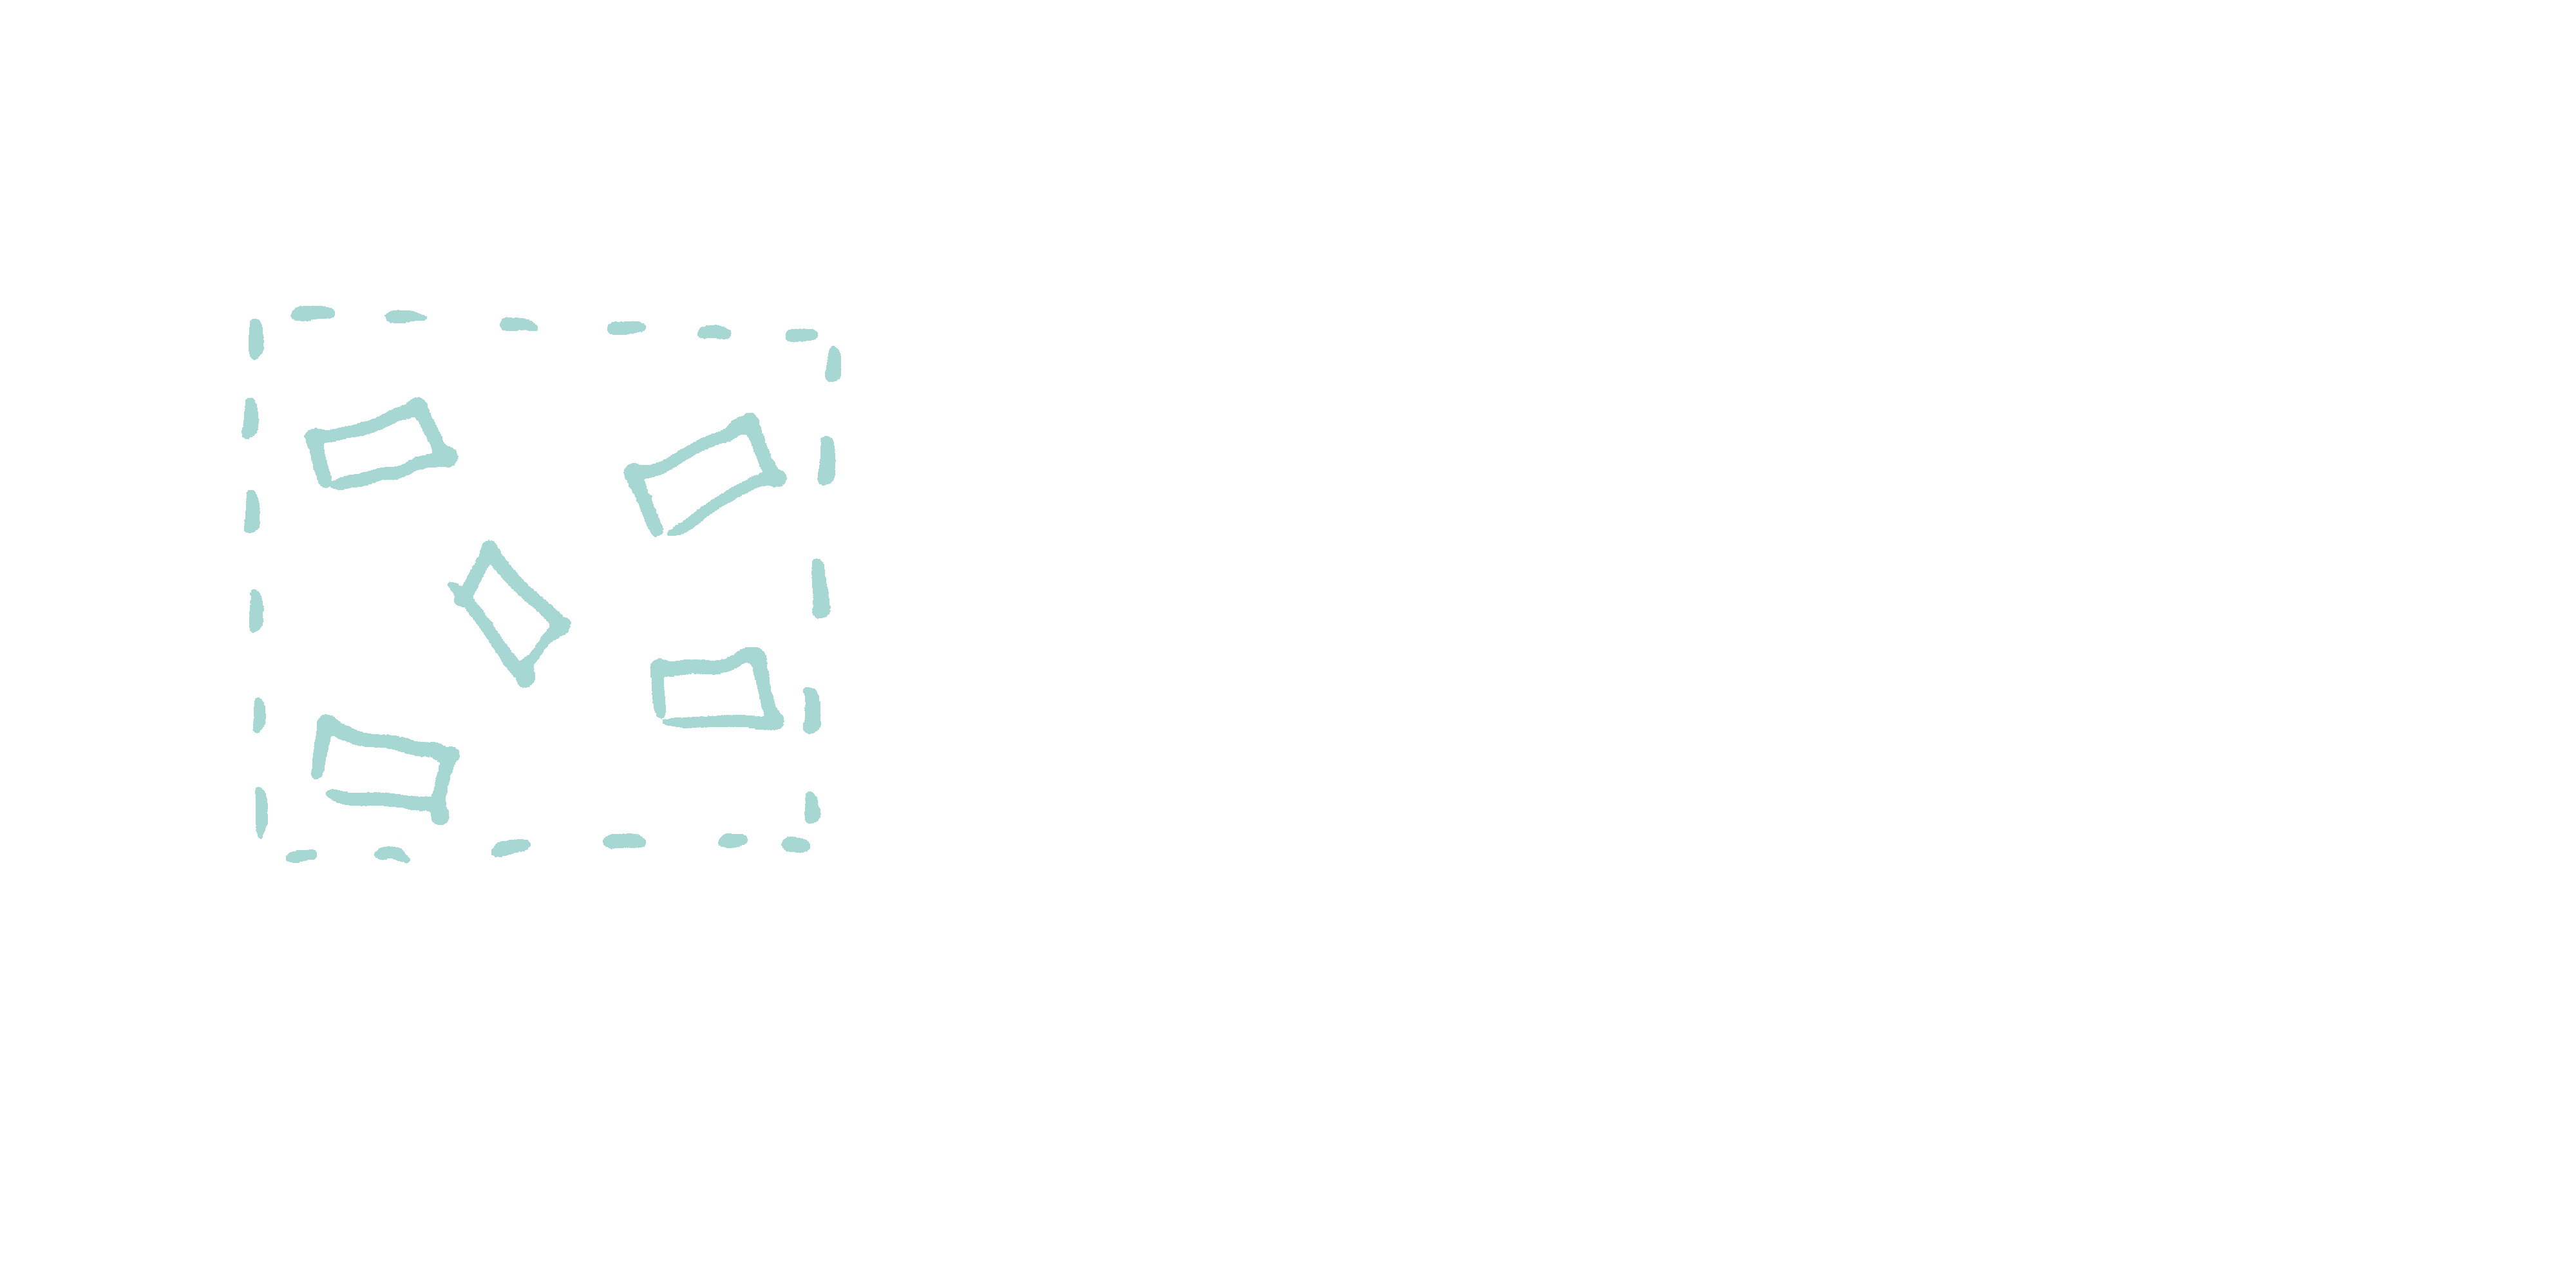
\includegraphics[height = 0.3\textheight]{../assets/images/block_1_mint}};
	
%	\draw[->, thick, color = highlight] (ledger.south east) + (-1, 1) -- (node.west);
%	\draw[->, thick, color = focus] (block1.west) + (0.5, 0) -- (client.north east);
	\draw[->, line width=0.5mm, color = focus] (block1.west) + (0.5, 0) -- node[midway, xshift=7, yshift=-7] {
\includegraphics[height = 0.05\textheight]{../assets/images/remove_red}} (client.north east);
	\draw[->, line width=0.5mm, color = highlight] (block2.west) + (0.5, 0) -- node[midway, xshift=7, yshift=7] {
\includegraphics[height = 0.05\textheight]{../assets/images/check_mint}} (client.south east);
	
	
\end{footnotesize}
	\end{tikzpicture}
\end{frame}
%%%

%%%
\begin{frame}{Relay Verified Blocks}
	
	\begin{tikzpicture}[scale=1, every node/.style={scale=1}]
		\begin{footnotesize}
	
	\node (ledger) at (0, 3) {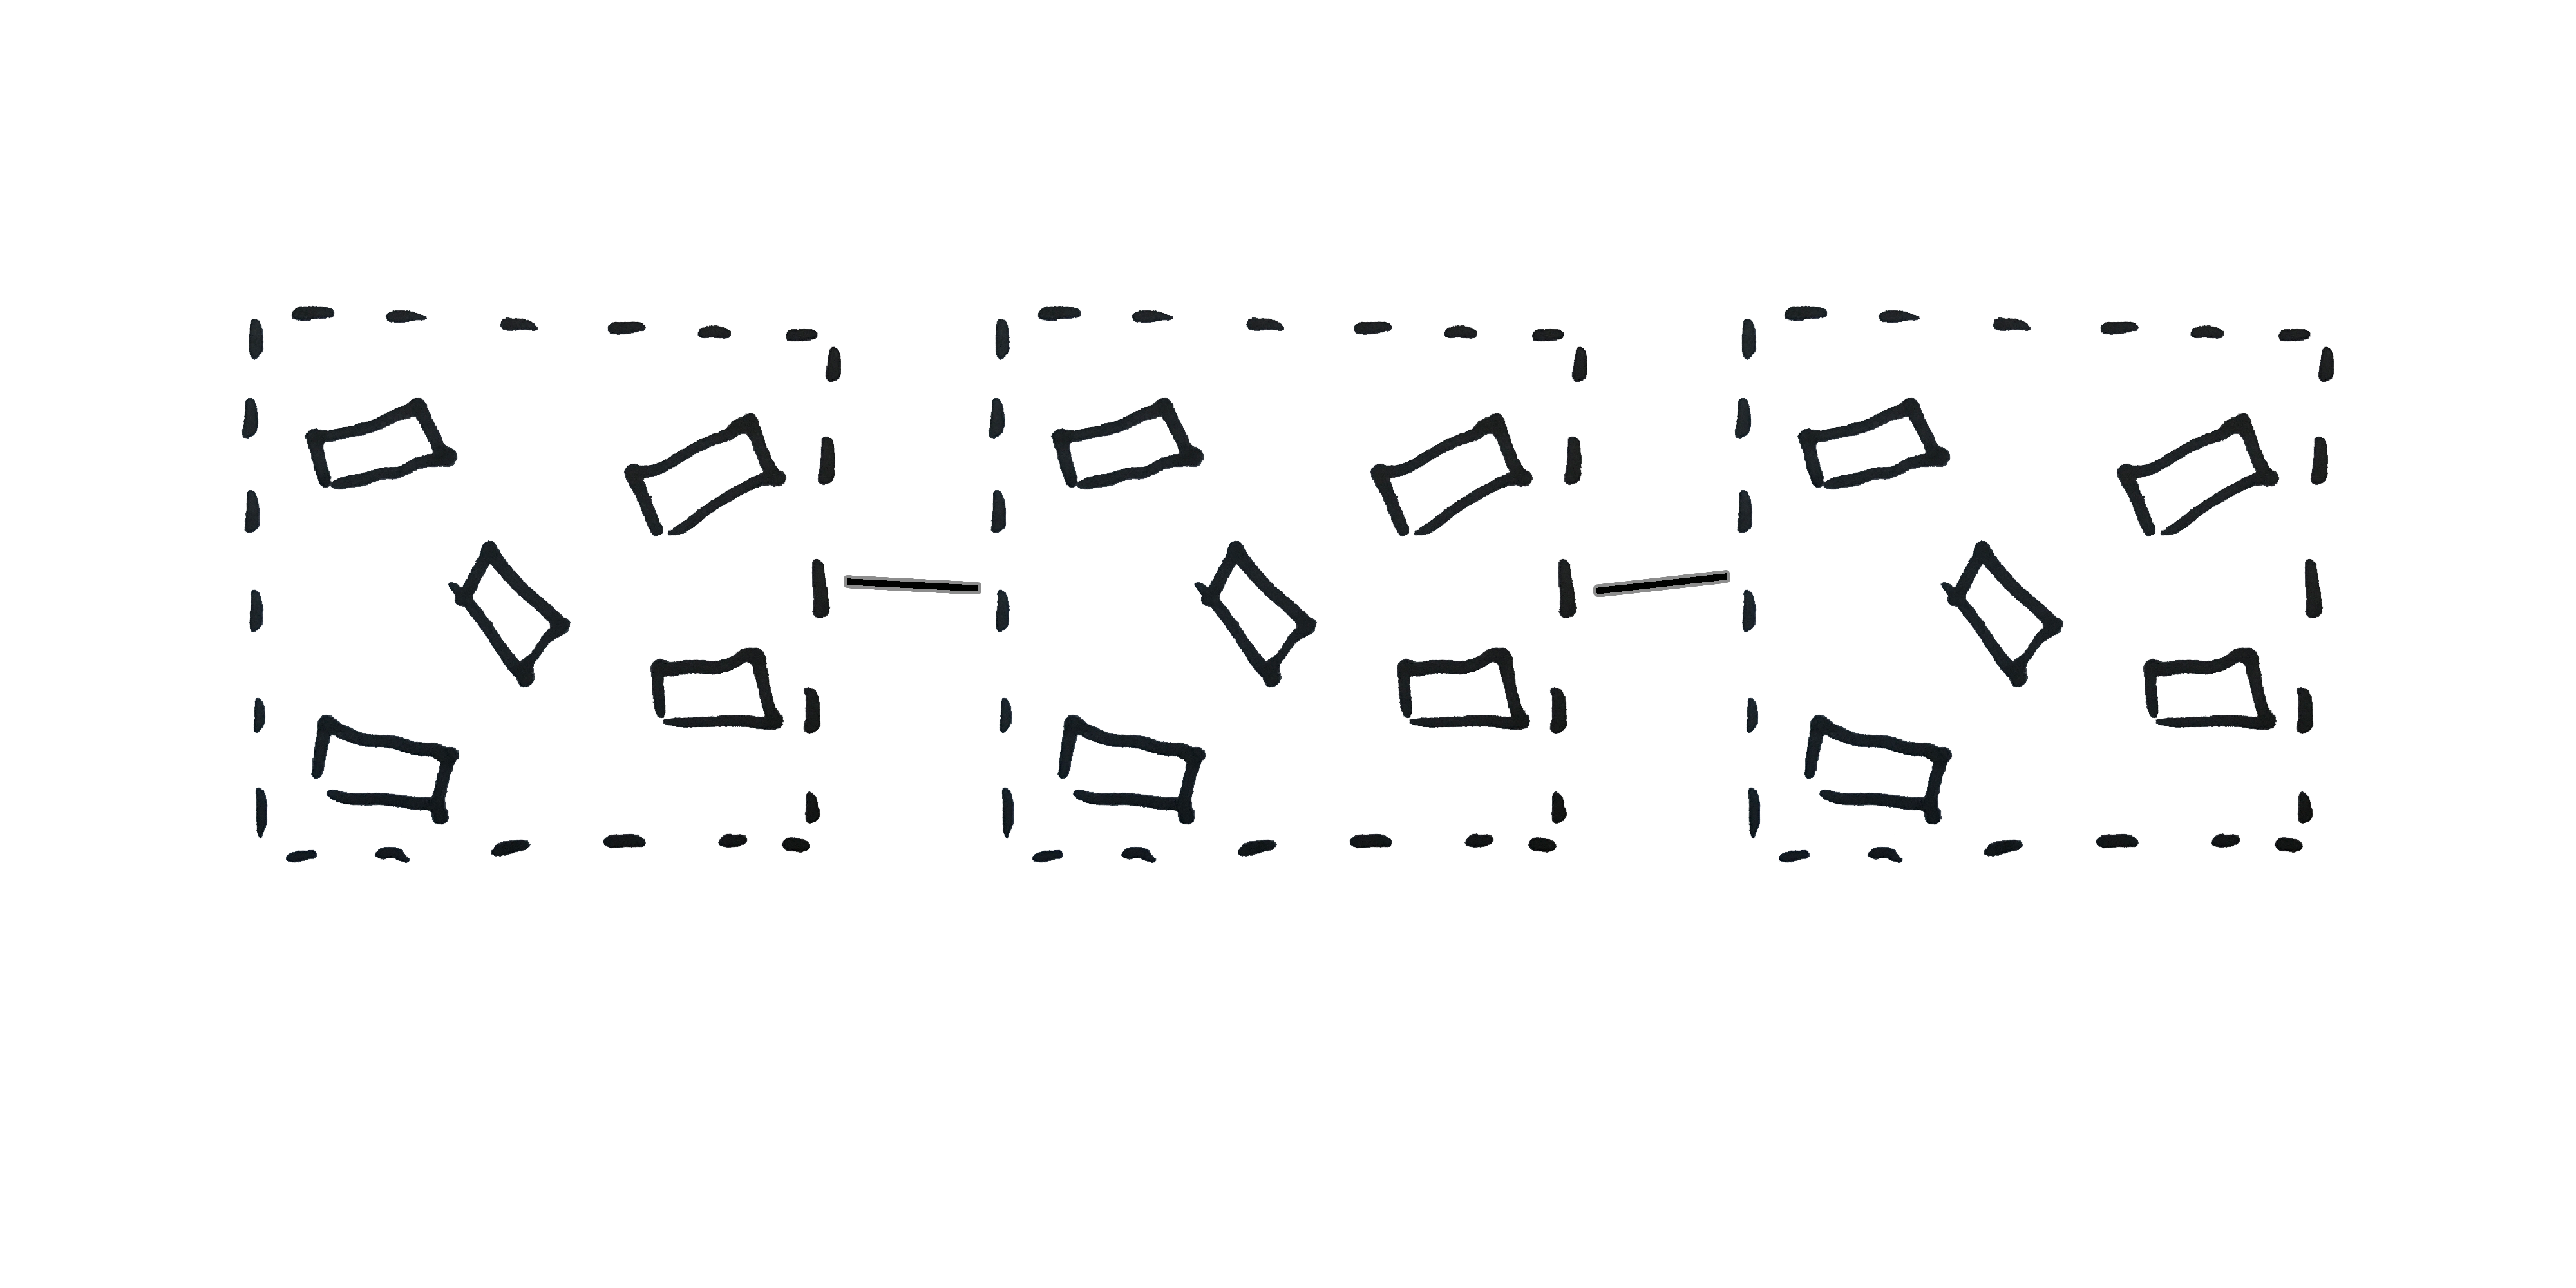
\includegraphics[height = 0.3\textheight, rotate = -90]{../assets/images/blocks_3}};
	\node (newblock) at (0, -1.8) {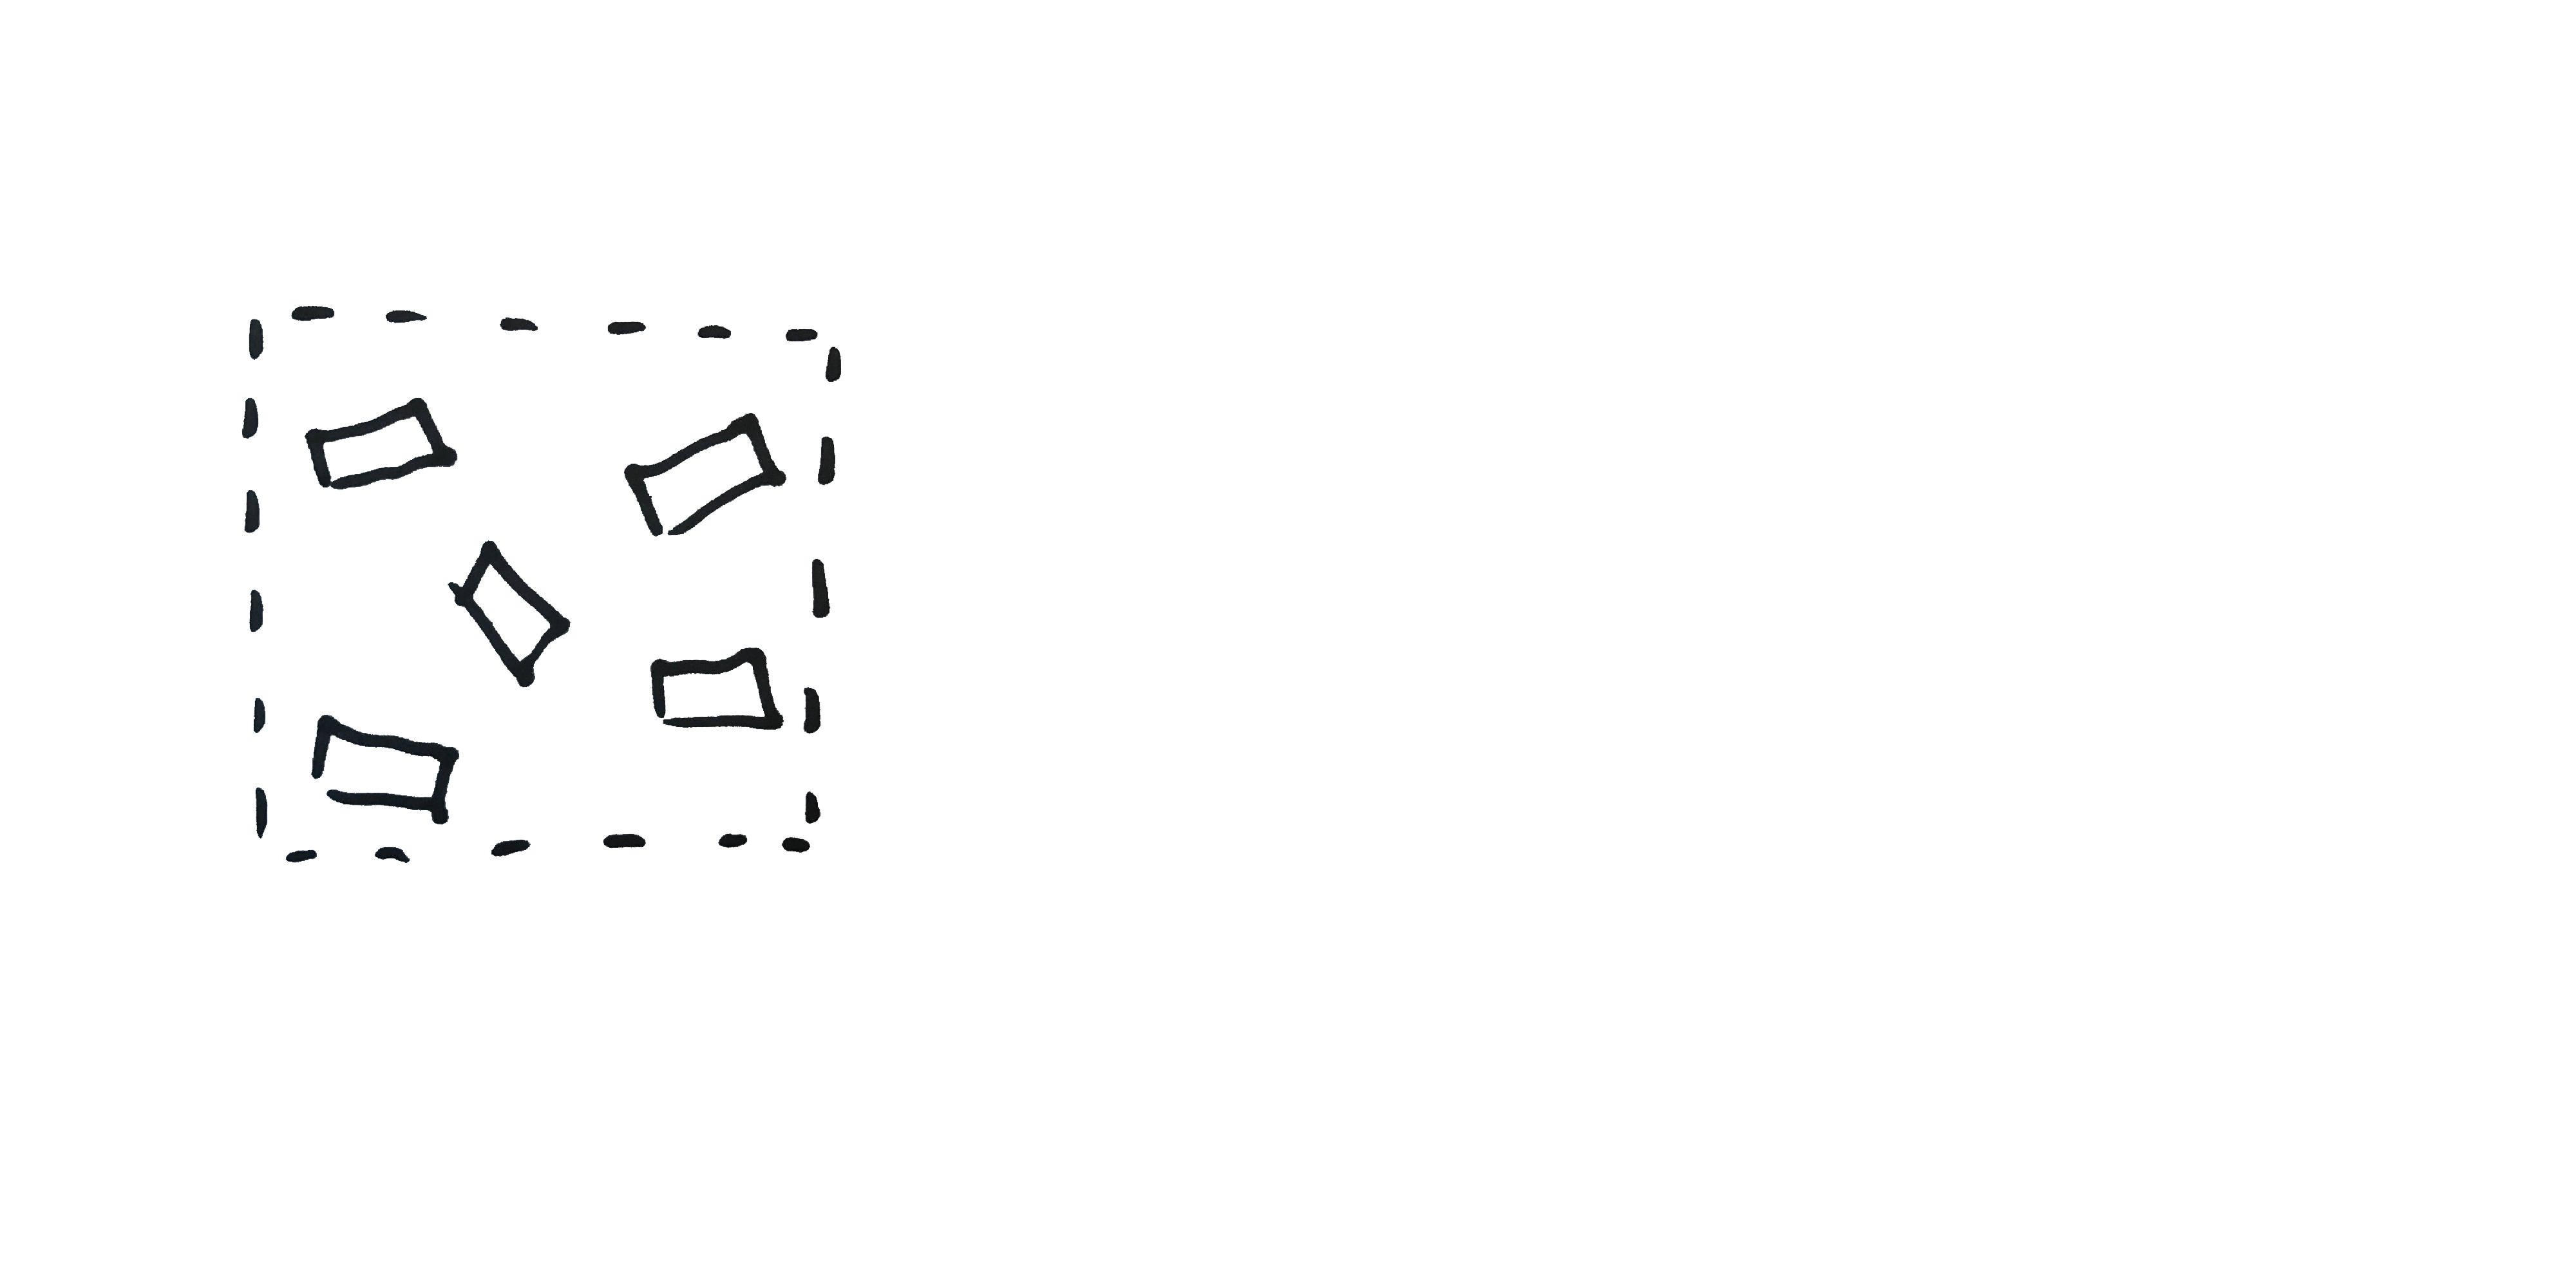
\includegraphics[height = 0.3\textheight, rotate = -90, decodearray={0.65 .8 0.84 .8 0.82 .8}]{../assets/images/block_1}};
	\draw[dashed, line width=0.35mm, color = highlight] (0.1, 0.8) -- (0.1, 0.4);
	\node (client) at (2, 2) {
\includegraphics[height = 0.2\textheight]{../assets/images/agents/handing_right}};
	\node (agent1) at (6, 4) {
\includegraphics[height = 0.2\textheight]{../assets/images/agents/reaching_left}};
	\node (agent2) at (6, 0) {
\includegraphics[height = 0.2\textheight]{../assets/images/agents/reaching_left}};
	\node (block) at (client) {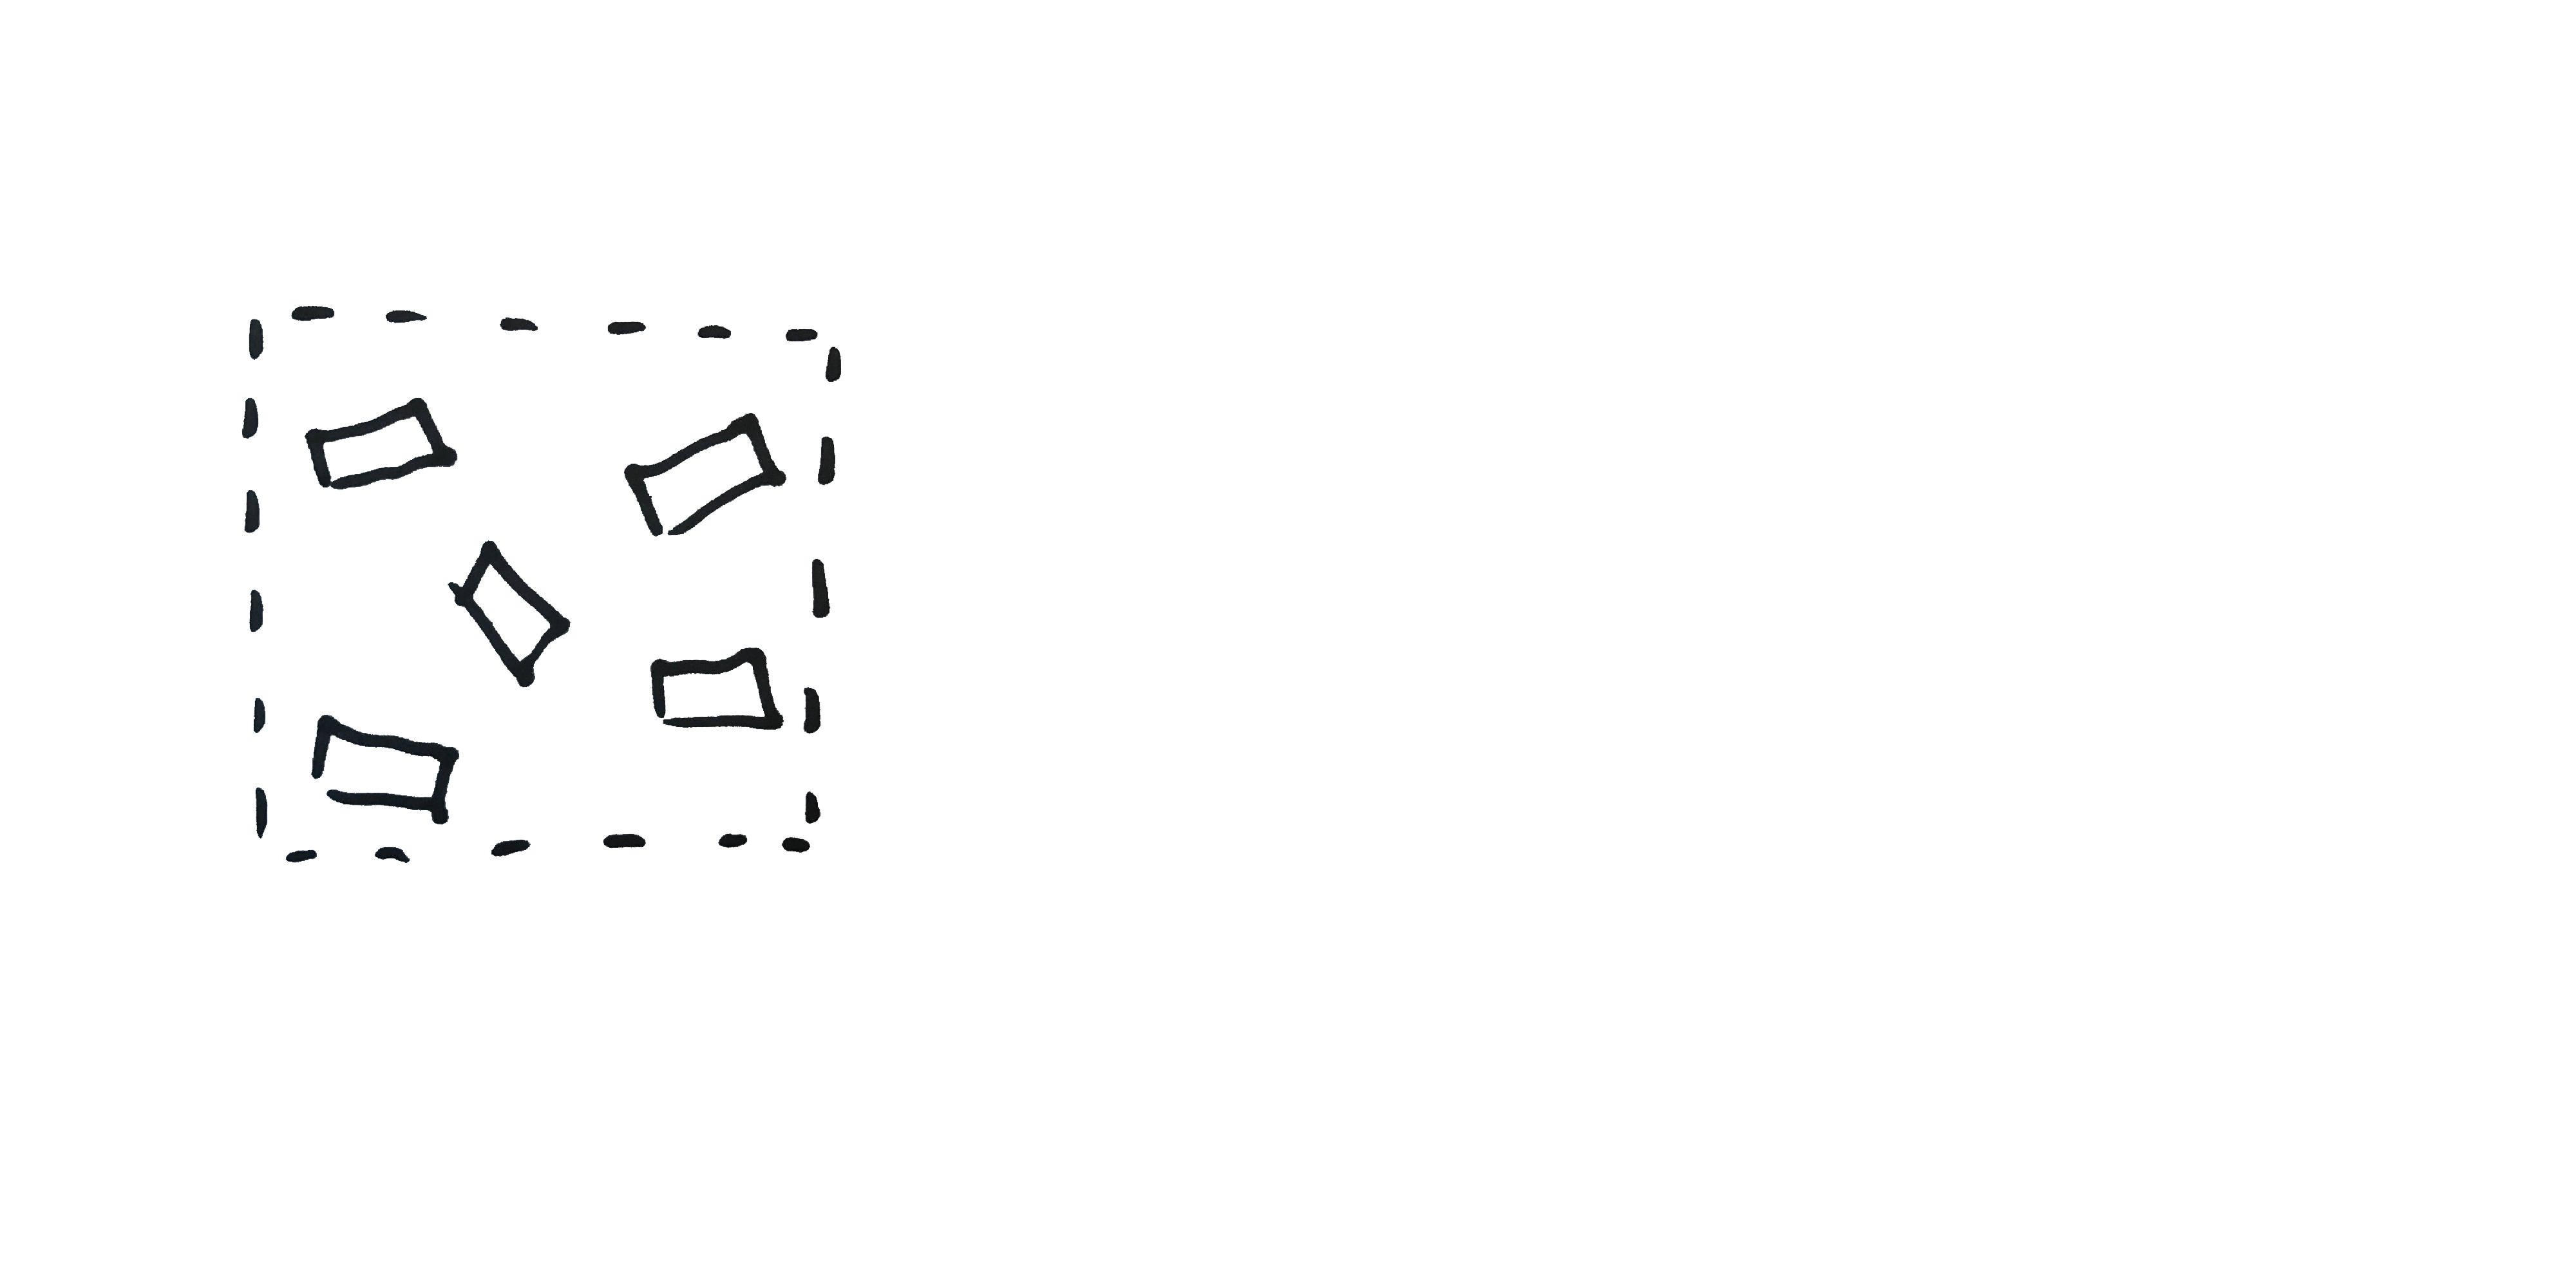
\includegraphics[height = 0.3\textheight, rotate = 180, decodearray={0.65 .8 0.84 .8 0.82 .8}]{../assets/images/block_1}};
	
	\draw[->, line width=0.5mm] (block.north east) + (-.8, -.8)-- (agent1.west);
	\draw[->, line width=0.5mm] (block.south east) + (-.8, .7)-- (agent2.west);
	
%	\draw[->, thick, color = highlight] (ledger.south east) + (-1, 1) -- (node.west);
%	\draw[->, thick, color = focus] (block1.west) + (0.5, 0) -- (client.north east);
%	\draw[->, thick, color = focus] (block1.west) + (0.5, 0) -- node[midway, xshift=7, yshift=-7] {
\includegraphics[height = 0.05\textheight, decodearray={1 1 0 1 0 1}]{../assets/images/remove}} (client.north east);
%	\draw[->, thick, color = highlight] (block2.west) + (0.5, 0) -- node[midway, xshift=7, yshift=7] {
\includegraphics[height = 0.05\textheight, decodearray={0.65 .8 0.84 .8 0.82 .8}]{../assets/images/check}} (client.south east);
	
	
\end{footnotesize}
	\end{tikzpicture}
\end{frame}
%%%

%%%
\begin{frame}{Exchange of Blocks}
	\begin{center}
		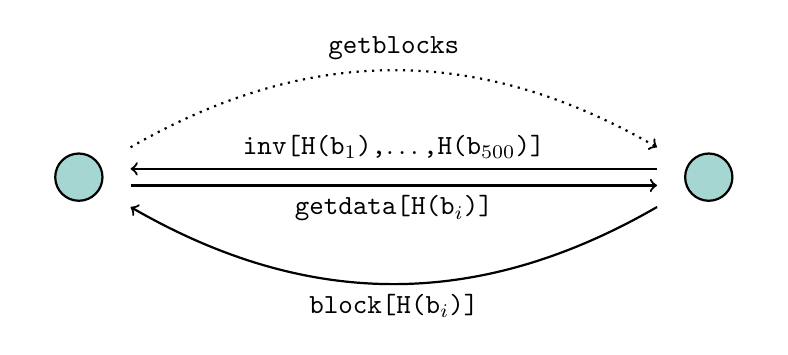
\begin{tikzpicture}[scale=1, every node/.style={scale=1}]
			\coordinate (1) at (-4, 0);
\coordinate (2) at (4, 0);

\node(node1)[minimum size = 1.3cm] at (1) {};
\node(node2)[minimum size = 1.3cm] at (2) {};

\filldraw[fill=highlight, thick](node1) circle (.3);
\filldraw[fill=highlight, thick](node2) circle (.3);

\draw[->, thick, dotted] (node1) edge [out=30, in=-210] node[midway,above] {\texttt{getblocks}} (node2);
\draw[<-, thick] ([yshift=3pt]node1.east) -- node[midway,above] {\texttt{inv[H(b$_1$),$\dots$,H(b$_{500}$)]}} ([yshift=3pt]node2.west);
\draw[->, thick] ([yshift=-3pt]node1.east) -- node[midway,below] {\texttt{getdata[H(b$_i$)]}} ([yshift=-3pt]node2.west);
\draw[<-, thick] (node1) edge [out=-30, in=210] node[midway,below] {\texttt{block[H(b$_i$)]}} (node2);
		\end{tikzpicture}
	\end{center}
\end{frame}
%%%

%%%
\begin{frame}{Exchange of Transactions}
	\begin{center}
		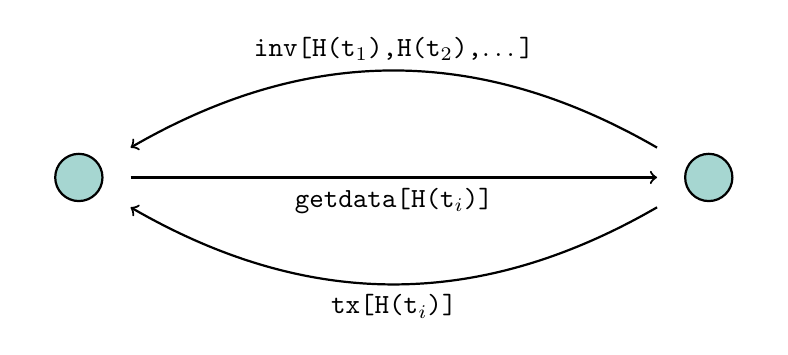
\begin{tikzpicture}[scale=1, every node/.style={scale=1}]
			\coordinate (1) at (-4, 0);
\coordinate (2) at (4, 0);

\node(node1)[minimum size = 1.3cm] at (1) {};
\node(node2)[minimum size = 1.3cm] at (2) {};

\filldraw[fill=highlight, thick](node1) circle (.3);
\filldraw[fill=highlight, thick](node2) circle (.3);

\draw[<-, thick] (node1) edge [out=30, in=-210] node[midway,above] {\texttt{inv[H(t$_1$),H(t$_2$),$\dots$]}} (node2);
\draw[->, thick] (node1.east) -- node[midway,below] {\texttt{getdata[H(t$_i$)]}} (node2.west);
\draw[<-, thick] (node1) edge [out=-30, in=210] node[midway,below] {\texttt{tx[H(t$_i$)]}} (node2);
		\end{tikzpicture}
	\end{center}
\end{frame}
%%%


%%%
\begin{frame}{Wallet Functionality}
	\centering
	\begin{tikzpicture}[scale=1, every node/.style={scale=1}]
		\begin{footnotesize}
	\coordinate (1) at (-4, 3);
	\coordinate (2) at (0, 3);
	\coordinate (3) at (4, 3);
	
	\coordinate (a) at (-5.3, 4);
	\coordinate (b) at (5.3, 1.5);
	\filldraw[fill=highlight] (a) rectangle (b);
	\node at (0, 4.25) {Security Layer};
	
	\node (keys) at (1) {
\includegraphics[height = 0.15\textheight]{../assets/images/key}};
	\node[below = 3pt] at (keys.south) {Keys};
	
	\node (balance) at (2) {
\includegraphics[height = 0.15\textheight]{../assets/images/bitcoin}};
	\node[below = 3pt] at (balance.south) {Balance};
	
	\node (gui) at (3) {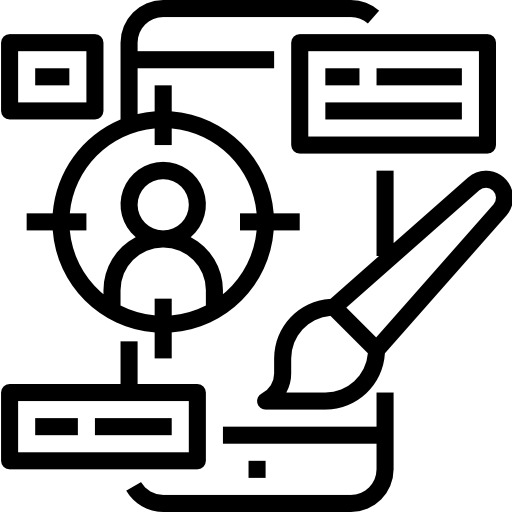
\includegraphics[height = 0.15\textheight]{../assets/images/ui}};
	\node[below = 3pt] at (gui.south) {GUI};
	
\end{footnotesize}
	\end{tikzpicture}
\end{frame}
%%%

%%%
\begin{frame}{Mining Functionality}
	\centering
	\begin{tikzpicture}[scale=1, every node/.style={scale=1}]
		\begin{footnotesize}
	\coordinate (1) at (-2, 3);
	\coordinate (2) at (2, 3);
	
	\node (compute) at (1) {
\includegraphics[height = 0.15\textheight]{../assets/images/compute}};
	\node[below = 3pt] at (compute.south) {Compute};
	
	\node (blocks) at (2) {
\includegraphics[height = 0.15\textheight]{../assets/images/block}};
	\node[below = 3pt] at (blocks.south) {Create Blocks};
	
\end{footnotesize}
	\end{tikzpicture}
\end{frame}
%%%

%%%
\begin{frame}{Pool Mining}
	\centering
	\begin{figure}[t]
		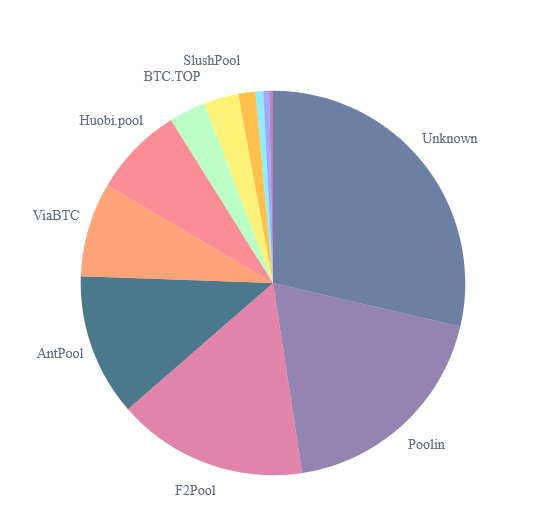
\includegraphics[height = 0.8\textheight]{../assets/images/mining_pools}
		
		Source: \link \url{https://blockchain.info/pools}, March 2021
	\end{figure}
\end{frame}
%%%

%%%
\begin{frame}{Node Distribution}
	\begin{figure}[t]
		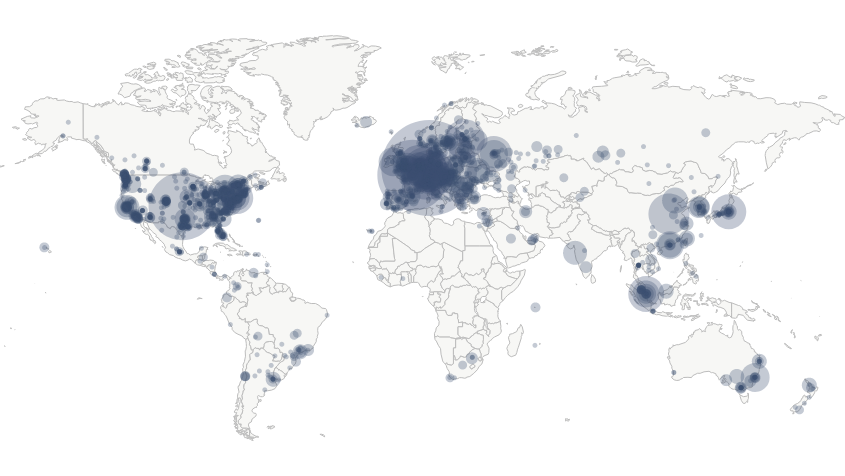
\includegraphics[width = 0.9\textwidth]{../assets/images/node_distribution}
		Source: \link \url{https://bitnodes.io/}, March 2021
	\end{figure}

	\begin{footnotesize}
		\begin{itemize}
			\item $\sim$ 50\% of nodes in Europe
			\item $\sim$ 20\% of nodes in the USA
		\end{itemize}
	\end{footnotesize}
	
\end{frame}
%%%

%%%
\begin{frame}{Historic Number of Full Nodes}
	\begin{description}
		\item[\textbf{Dec 2013:}] $\sim$ 15,500 full nodes
		\item[\textbf{Dec 2015:}] $\sim$ 5,500 full nodes
		\item[\textbf{Mar 2017:}] $\sim$ 6,500 full nodes
		\item[\textbf{Mar 2019:}] $\sim$ 10,400 full nodes
		\item[\textbf{Mar 2021:}] $\sim$ 10,200 full nodes
	\end{description}	
		
	\vspace{1 cm}
	
	Motivations for running a full node:
	\begin{itemize}
		\item Independence
		\item Direct access to data
	\end{itemize}
	
\end{frame}
%%%

%%%
%\begin{frame}{Network Partitions}
%	%% Leave out for now
%	\centering
%	\begin{tikzpicture}[scale=1, every node/.style={scale=1}]
%		
% Network
\node (agenta) at (1,2.8) {\includegraphics[width = 0.6 cm]{../assets/images/agents/avatar_rand3.png}};
\node (agentb) at (0.5,1) {\includegraphics[width = 0.6 cm]{../assets/images/agents/avatar_rand4.png}};
\node (agentc) at (3,2.1) {\includegraphics[width = 0.6 cm]{../assets/images/agents/avatar_rand5.png}};
\node (agentd) at (2.8,0) {\includegraphics[width = 0.6 cm]{../assets/images/agents/avatar_rand1.png}};
\node (agente) at (5,4.3) {\includegraphics[width = 0.6 cm]{../assets/images/agents/avatar_rand2.png}};	
\node (agentf) at (5.1,1.1) {\includegraphics[width = 0.6 cm]{../assets/images/agents/avatar_rand3.png}};
\node (agentg) at (7.5,3.8) {\includegraphics[width = 0.6 cm]{../assets/images/agents/avatar_rand4.png}};
\node (agenth) at (6.7,0.4) {\includegraphics[width = 0.6 cm]{../assets/images/agents/avatar_rand5.png}};

% Network flow
\draw[<->, thick, dashed]	(agenta.south) -- (agentb.north);
\draw[<->, thick, dashed] 	(agenta.east) -- (agente.west);
\draw[<->, thick, dashed]	(agenta.south east) -- (agentc.west);
\draw[<->, thick, dashed]	(agente.south west) -- (agentc.north east);
\draw[<->, thick, dashed]	(agentc.south west) -- (agentb.east);
\draw[<->, thick, dashed]	(agentg.south west) -- (agentf.north east);
\draw[<->, thick, dashed]	(agentg.south) -- (agenth.north);
\draw[<->, thick, dashed]	(agentf.south west) -- (agentd.east);
\draw[<->, thick, dashed]	(agentf.south east) -- (agenth.west);
\draw[<->, thick, dashed]	(agenth.south west) -- (agentd.east);
\draw[<->, thick, dashed]	(agentg.west) -- (agentd.north east);

%	\end{tikzpicture}
%\end{frame}
%%%


%%%
\begin{frame}{Extended Network}
	\centering
	\begin{tikzpicture}[scale=1, every node/.style={scale=1}]
		
% Network
\node (agenta) at (1,2.8) {\includegraphics[width = 0.6 cm]{../assets/images/agents/avatar_rand3.png}};
\node (agentb) at (0.5,1) {\includegraphics[width = 0.6 cm]{../assets/images/agents/avatar_rand4.png}};
\node (agentc) at (3,2.1) {\includegraphics[width = 0.6 cm]{../assets/images/agents/avatar_rand5.png}};
\node (agentd) at (2.8,0) {\includegraphics[width = 0.6 cm]{../assets/images/agents/avatar_rand1.png}};
\node (agente) at (5,4.3) {\includegraphics[width = 0.6 cm]{../assets/images/agents/avatar_rand2.png}};	
\node (agentf) at (5.1,1.1) {\includegraphics[width = 0.6 cm]{../assets/images/agents/avatar_rand3.png}};
\node (agentg) at (7.5,3.8) {\includegraphics[width = 0.6 cm]{../assets/images/agents/avatar_rand4.png}};
\node (agenth) at (6.7,0.4) {\includegraphics[width = 0.6 cm]{../assets/images/agents/avatar_rand5.png}};

% Network flow
\draw[<->, thick, dashed]	(agenta.south) -- (agentb.north);
\draw[<->, thick, dashed] 	(agenta.east) -- (agente.west);
\draw[<->, thick, dashed]	(agenta.south east) -- (agentc.west);
\draw[<->, thick, dashed]	(agente.south west) -- (agentc.north east);
\draw[<->, thick, dashed]	(agente.south) -- (agentf.north);
\draw[<->, thick, dashed]	(agente.east) -- (agentg.west);
\draw[<->, thick, dashed]	(agentc.south west) -- (agentb.east);
\draw[<->, thick, dashed]	(agentc.south) -- (agentd.north);
\draw[<->, thick, dashed]	(agentc.south east) --  (agentf.west);
\draw[<->, thick, dashed]	(agentg.south west) -- (agentf.north east);
\draw[<->, thick, dashed]	(agentg.south) -- (agenth.north);
\draw[<->, thick, dashed]	(agentb.south east) -- (agentd.west);
\draw[<->, thick, dashed]	(agentf.south west) -- (agentd.east);
\draw[<->, thick, dashed]	(agentf.south east) -- (agenth.west);
\draw[<->, thick, dashed]	(agenth.south west) -- (agentd.east);

% Extended Network
\node (agent1) at (7.5, 5.5) {\includegraphics[width = 0.6 cm]{../assets/images/agents/avatar_rand5_gray}};
\node (agent2) at (9.2, 5) {\includegraphics[width = 0.6 cm]{../assets/images/agents/avatar_rand4_gray}};
\node (agent3) at (8.8, 2.5) {\includegraphics[width = 0.6 cm]{../assets/images/agents/avatar_rand3_gray}};

\node (key1) at (agentg.east) {\includegraphics[width = 0.3 cm]{../assets/images/key_gray}};
\node[xshift=0.3 cm] (key2) at (agentg.east) {\includegraphics[width = 0.3 cm]{../assets/images/key_gray}};
\node[xshift=0.6 cm] (key3) at (agentg.east) {\includegraphics[width = 0.3 cm]{../assets/images/key_gray}};

\node (agent4) at (1, -1) {\includegraphics[width = 0.6 cm]{../assets/images/agents/avatar_rand5_gray}};
\node (agent5) at (4.1, -1.7) {\includegraphics[width = 0.6 cm]{../assets/images/agents/avatar_rand5_gray}};

\node (key4) at (agent4.west) {\includegraphics[width = 0.3 cm]{../assets/images/key_gray}};
\node (key5) at (agent5.west) {\includegraphics[width = 0.3 cm]{../assets/images/key_gray}};

\color{lightgray}
\draw[<->, thick, dashed]	(agentg.north) -- (agent1.south);
\draw[<->, thick, dashed]	(agentg.north east) -- (agent2.south west);
\draw[<->, thick, dashed]	(agentg.south east) -- (agent3.north west);

\draw[<->, thick, dashed]	(agentd.south west) -- (agent4.east);
\draw[<->, thick, dashed]	(agentd.south east) -- (agent5.north west);
	\end{tikzpicture}
\end{frame}
%%%

%%%
\begin{frame}{Mobile Options}

	Running a node on a mobile device is challenging.
	\vspace{0.1cm}
	
	\begin{center}
		\begin{tikzpicture}[scale=1, every node/.style={scale=1}]
			\coordinate (1) at (-3, 0);
\coordinate (2) at (0, 0);
\coordinate (3) at (3, 0);

\node at (1) {\includegraphics[height = 0.1\textheight]{../assets/images/harddisk}};
\node[below = 14pt] at (1) {Storage Capacity};

\node at (2) {\includegraphics[height = 0.1\textheight]{../assets/images/connectivity}};
\node[below = 14pt] at (2) {Bandwidth};

\node at (3) {\includegraphics[height = 0.1\textheight]{../assets/images/battery}};
\node[below = 14pt] at (3) {Battery};
		\end{tikzpicture}
	\end{center}
	\vspace{0.8 cm}

	There are compromises to retain some independence.
	\vspace{0.1cm}
	
	\begin{center}
		\begin{tikzpicture}[scale=1, every node/.style={scale=1}]
			\coordinate (1) at (-2, 0);
\coordinate (2) at (2, 0);

\node at (1) {\includegraphics[height = 0.1\textheight]{../assets/images/wallet}};
\node[below = 14pt] at (4) {SPV Wallet};

\node at (2) {\includegraphics[height = 0.1\textheight]{../assets/images/smarthome}};
\node[below = 14pt] at (5) {Connect to Node};

		\end{tikzpicture}
	\end{center}

\end{frame}
%%%

%%%
%\begin{frame}{Recommended Literature}
%	Nothing so far, paper will be added when released
%\end{frame}
%%%

\end{document}